\documentclass[12pt,a4paper]{article}
\title{%
  Øving 4 \\
  \large IELET1001 - Elektroteknikk \\
  }
\author{Gunnar Myhre, BIELEKTRO}

\usepackage[utf8]{inputenc}
\usepackage[norsk]{babel}
\usepackage[siunitx]{circuitikz}
\usepackage{pgfplots}
\usepackage{amsmath}

\setlength\parindent{0pt}

\begin{document}
  \maketitle
    
  \section{Oppgåve 1}
    Vi veit at utgongssignalet er gitt ved $v_o=A\cdot v_s$. For $A = 15$ får vi:
    \begin{center}
      \begin{tabular}{ |c|c|c|c|c|c|c|c| }
        \hline
        $t [s]$ & $0$ & $0,5^-$ & $0,5^+$ & $1$ & $1,5^-$ & $1,5^+$ & $2$ \\
        \hline
        $v_{in}[mV]$ & $0$ & $50$ & $-100$ & $-150$ & $0$ & $50$ & $0$ \\
        \hline
        $v_{o}[mV]$ & $0$ & $750$ & $-1500$ & $-2250$ & $0$ & $750$ & $0$ \\
        \hline
      \end{tabular}
    \end{center}

    \begin{center}
      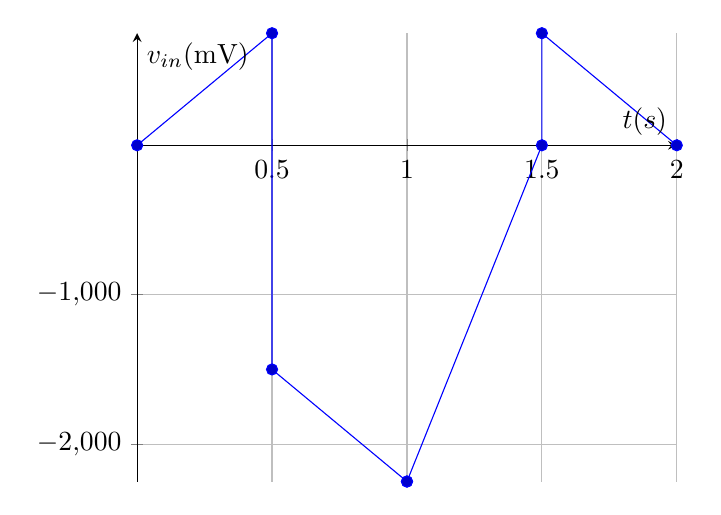
\begin{tikzpicture}
        \begin{axis}[axis lines=middle,grid=both,xlabel=$t(s)$,ylabel=$v_{in}$(mV)]
          \addplot coordinates{
            (0,0)        (0.5, 750)
            (0.5, -1500) (1,-2250)
            (1, -2250)   (1.5, 0)
            (1.5, 750)   (2, 0)
          };
        \end{axis}
      \end{tikzpicture}
    \end{center}

  \section{Oppgåve 2}
    \begin{itemize}
      \item $v^+ = v^-$ i ein ideell op-amp.
      \item $i^+ = i^- = 0$ i ein ideell op-amp.
      \item Utgongsstraumen $i_o$ er avhengig av kretsen som op-ampen inngår i. For eksempel
        vil $i_o$ for ein ikkje-inverterande forsterkar vere gitt ved
        $i_o = \frac{v_o-v_{in}}{R_F}+\frac{v_o}{R_L}$
    \end{itemize}

  \section{Oppgåve 3}
    \begin{itemize}
      \item Straumkjelda til venstre sørger for at $I_1 = 2,85mA$
      \item Sidan dette er ein ideell op-amp er $I_2 = 0A$
      \item Derfor (pga KCL) må $I_3 = 2,85mA$
    \end{itemize}

  \section{Oppgåve 4}
    \begin{center}
      \begin{circuitikz}[american] \draw
        (0,0) to[R, l=$R_1$] (4,0)
              to[R, l=$R_2$] (8,0)
              to[R, l=$R_o$] (8, -2)
              to[cV, l=$A_0v_e$] (8, -4) -- (4, -4) -- (0, -4)
              to[V, l=$v_s$, invert] (0,0)
        (4, -4) to[R, l=$R_i$, v=$v_e$] (4, 0)
        (4, -4) node[ground]{} (4, -5)

        (8,0)  to[short, *-o] (10,0)
        (8,-4) to[short, *-o] (10,-4)
        (10, 0) to[open, v=$v_o$] (10, -4)
        
        (4,0) node[label={[font=\footnotesize]100:$-v_e$}] {}
        ;
      \end{circuitikz}
    \end{center}
    \subsection{a)}
      Setter opp KCL i node $-v_e$. Vi setter $R_o = 0$ som gitt i oppgåveteksten
      (m.a.o. tenker på den som ein kortslutning).
      \begin{equation}
        \frac{-v_e-v_s}{R_1} + \frac{-v_e}{R_i} + \frac{-v_e-A_0v_e}{R_2} = 0
      \end{equation}
      forenkler algebraisk for å finne uttrykk for $A_0$
      \begin{equation}
        A_0 = -\frac{R_2(v_e+v_s)}{R_1v_e} - \frac{R_2}{R_i} - 1
      \end{equation}

    \subsection{b)}
      Setter inn verdiar for $R_1 = 15\si{\ohm}$, $R_2 = 10\si{\ohm}$, $R_i = 24\si{\ohm}$
      og $A_0 = 15$
      \begin{equation}
        15 = -\frac{10(v_e+v_s)}{15v_e} - \frac{10}{24} - 1
      \end{equation}
      får uttrykk for proporsjonen mellom $v_s$ og $v_e$
      \begin{equation}
        v_s = -25,625v_e
      \end{equation}
      om vi setter dette inn i formelen for forsterking $v_o = A_0 \cdot v_s 
      \Rightarrow A = \frac{v_o}{v_s}$ finner vi
      \begin{equation}
        A = \frac{A_0v_e}{-25,625v_e} = -\frac{15}{25,625} = -0,5853
      \end{equation}
      Sidan forsterkingskoeffisienten A er negativ har vi ein inverterande forsterkar

    \subsection{c)}
      Ein inverterande forsterkar med ideell op-amp vil ha ein forsterking på
      $-\frac{R_F}{R_I}$. Om vi setter inn for $R_1$ og $R_2$ får vi
      \begin{equation}
        -\frac{10}{15} = -\frac{2}{3} \approx -0,66
      \end{equation}
      altså lågare enn den ikkje-ideelle op-ampen var i stand til.


  \section{Oppgåve 5}
    Gjør KCL i $v^-$ på op-ampen
    \begin{equation}
      \frac{0-v_s}{5\si{\kilo\ohm}} + \frac{0-v_o}{25\si{\kilo\ohm}} = 0
    \end{equation}
    finner uttrykk for $v_s$
    \begin{equation}
      v_s = -\frac{1}{5}v_o
    \end{equation}
    sidan $A = \frac{v_o}{v_s}$ finner vi
    \begin{equation}
      A = -\frac{v_o}{\frac{1}{5}v_o} = -5
    \end{equation}

  \section{Oppgåve 6}
    Bruker KCL i inngongsnoden til op-ampen $v^-$
    \begin{equation}
      \frac{0-1V}{10\si{\kilo\ohm}} + \frac{0-2V}{20\si{\kilo\ohm}} +
      \frac{0+3V}{30\si{\kilo\ohm}} + \frac{0-v_o}{30\si{\kilo\ohm}} = 0
    \end{equation}
    som kan forenklast til
    \begin{equation}
      -3V - 3V + 3V = V_o \Rightarrow V_o = -3V
    \end{equation}

  \section{Oppgåve 7}
    Setter opp KCL i dei to inngongsnodane til op-ampen, $v^+$ og $v^-$. Spenninga i desse
    nodane er den same pga. ideell op-amp. Kaller denne spenninga $v$
    \begin{equation}
      KCL^-: \frac{v-3V}{2\si{\kilo\ohm}} + \frac{v-v_o}{8\si{\kilo\ohm}} = 0
    \end{equation}
    \begin{equation}
      KCL^+: \frac{v-3V}{5\si{\kilo\ohm}} + \frac{v}{10\si{\kilo\ohm}} = 0
    \end{equation}
    løyser likningssettet og finner $v_o = -2V$. Setter opp KCL i utgongen for å finne $I_o$
    \begin{equation}
      \frac{v_o-v}{8\si{\kilo\ohm}} + \frac{v_o}{4\si{\kilo\ohm}} - I_o = 0 
      \Rightarrow I_o = -1\si{\milli\ampere}
    \end{equation}

  \section{Oppgåve 8}
    Setter opp KCL i inngongsnoden til op-ampen. Vi veit at $v^- = v^+ = 3V$
    \begin{equation}
      \frac{3V-9V}{2\si{\kilo\ohm}} + \frac{3V}{1\si{\kilo\ohm}} +
      \frac{3V-V_o}{2\si{\kilo\ohm}} = 0
    \end{equation}
    løyser og får
    \begin{equation}
      3V - 9V + 6V + 3V = V_o \Rightarrow V_o = 3V
    \end{equation}

  \newpage

  \section{Oppgåve 9}
    \begin{center}
      \begin{circuitikz}[american] \draw
        (0, 0) to[R, l=5<\kilo\ohm>, -*] (3, 0) -- (4,0)
              node[op amp, anchor=-](OA){} (8,0)
        (OA.+) -- (3,-0.98)
               to[R, l=30<\kilo\ohm>] (3, -4) -- (1, -4)
               node[ground]{} (1, -5)
        (1, -4) -- (0, -4)
               to[V, l=2<\volt>, invert] (0,0)
        (OA.out) to[short, -o, l=$v_2$] (8, -0.49)
        (3, 0) -- (3, 1.5)
               to[R, l=20<\kilo\ohm>, i>_=$I_{v2}$] (7, 1.5) -- (7, -0.49)

        (3,0) node[below]{$v_i$}
        ;
      \end{circuitikz}
    \end{center}
    Vi veit at det ikkje går nokon straum inn i op-ampen, derfor er
    \begin{equation}
      I_{v2} = \frac{2V}{5\si{\kilo\ohm}} = 2,5mA
    \end{equation}
    spenninga i $v_2$ er derfor
    \begin{equation}
      v_2 = \frac{2V\cdot 20\si{\kilo\ohm}}{5\si{\kilo\ohm}} = 8V
    \end{equation}
    Vi kan se bort ifrå op-ampen med output i $V_1$. $V_1 = 3V$
    \begin{center}
      \begin{circuitikz}[american] \draw
        (0, 0) to[R, l=10<\kilo\ohm>] (3, 0) -- (4,0)
              node[op amp, noinv input up, anchor=+](OA){} (8,0)
        (OA.-) -- (3,-0.98) -- (3, -3)
               to[R, l=30<\kilo\ohm>] (3, -5) -- (1, -5)
               node[ground]{} (1, -6)
        (1, -5) -- (0, -5)
               to[V, l=3<\volt>, invert] (0,0)
        (OA.out) to[short, -o, l=$v_3$] (8, -0.49)
        (3,-3) to[R, l=50<\kilo\ohm>] (7, -3) -- (7, -0.49)

        (3,-1) node[left]{$v_i$}
        ;
      \end{circuitikz}
    \end{center}
    vi veit at spenninga i $v_i$ må vere 3V. Det går ingen straum igjennom 10k-motstanden
    og ein ideell op-amp sørger for at spenninga er lik på dei to inngongsterminalane.
    \begin{equation}
      KCL_{v_i}: \frac{3V}{30\si{\kilo\ohm}} + \frac{3V-v_3}{50\si{\kilo\ohm}} = 0
    \end{equation}
    finner at $v_3 = 8V$
    \begin{center}
      \begin{circuitikz}[american] \draw
        (-2, 1) to[short, o-, l=$-8V$] (-1, 1)
                to[R, l=40<\kilo\ohm>] (2, 1) -- (2, 0)
        (-2, -1) to[short, o-, l=$8V$] (-1, -1)
                to[R, l=80<\kilo\ohm>] (2, -1) -- (2, 0) -- (3, 0) -- (4,0)
              node[op amp, anchor=-](OA){} (8,0)
        (OA.+) -- (3,-0.98)
               to[R, l=20<\kilo\ohm>] (3, -4)
               node[ground]{} (1, -5)
        (OA.out) to[short, -o, l=$v_o$] (8, -0.49)
        (3, 0) -- (3, 1.5)
               to[R, l=100<\kilo\ohm>] (7, 1.5) -- (7, -0.49)

        (3,0) node[below]{$v_i$}
        ;
      \end{circuitikz}
    \end{center}
    setter opp KCL i noden $v_i = 0V$
    \begin{equation}
      \frac{0-8V}{80\si{\kilo\ohm}} + \frac{0-(-8V)}{40\si{\kilo\ohm}} + 
      \frac{0-v_o}{100\si{\kilo\ohm}} = 0
    \end{equation}
    finner $v_o = 10V$ \\

    Ein lettare måte å løyse oppgåva på ville ha vore å identifisere karakteristiske
    forsterkarar i kretsen (inverterande, ikkje-inverterande og summerande), og bruke
    formlane som vi kjenner frå før:
    \begin{itemize}
      \item Inverterande forsterkar: $v_2 = -\frac{20}{5}2V = -8V$
      \item Ikkje-inverterande forsterkar: $v_3 = (1 + \frac{50}{30})3V = 8V$
      \item Summerande forsterkar: $v_o = -(8V\frac{100}{80}-8V\frac{100}{40}) = 10V$
    \end{itemize}


  \section{Oppgåve 10}
    Kaller spenninga i inngongane til den høgre op-ampen for $v_2$. Spenninga i inngongen
    til op-ampen til venstre er 0V. Vi finner første likning ved å sette opp KCL i
    minus-inngongen til op-ampen til venstre.
    \begin{equation}
      \frac{0-v_1}{5\si{\kilo\ohm}} + \frac{0-v_2}{10\si{\kilo\ohm}} + 
      \frac{0-v_o}{4\si{\kilo\ohm}} = 0
    \end{equation}
    setter opp KCL i minus-inngongen til den høgre op-ampen
    \begin{equation}
      \frac{v_2}{10\si{\kilo\ohm}} + \frac{v_2-v_o}{2\si{\kilo\ohm}} = 0
    \end{equation}
    forenkler til likningene
    \begin{itemize}
      \item $-2v_1 -v_2 -\frac{10}{4}v_o = 0$
      \item $v_2 = \frac{5}{6}v_o$
    \end{itemize}
    løyser likningssettet for $v_1$ og $v_o$ og finner $\frac{v_o}{v_1}=-\frac{24}{40}=-0,6$

  \section{Oppgåve 11}
    Om vi teikner skjemaet på nytt er det lettare å sjå at dette er ein
    inverterande forsterkar.
    \begin{center}
      \begin{circuitikz}[american] \draw
        (0, 0) to[R, l=$R_1$, -*] (3, 0) -- (4,0)
              node[op amp, anchor=-](OA){} (8,0)
        (OA.+) -- (3,-0.98)
               node[ground]{} (1, -5)
        (OA.out) to[short, -o, l=$v_o$] (8, -0.49)
        (3, 0) -- (3, 1.5)
               to[R, l=$R_2$] (7, 1.5) -- (7, -0.49)

        (0, 0) to[short, -o, l=$v_s$] (-1, 0)
        ;
      \end{circuitikz}
    \end{center}
    Då veit vi at $v_o = -\frac{R_2}{R_1}v_s$. For at $-\frac{R_2}{R_1} = -110$ må $R_2$
    vere 110 gonger større enn $R_1$. Vi kan f.eks gjere slik:
    \begin{itemize}
      \item $R_1 = 2\si{\kilo\ohm}$
      \item $R_2 = 220\si{\kilo\ohm}$
    \end{itemize}

  \section{Oppgåve 12}
    Her er det uklart kva oppgåva meiner med eit invertert spenningssignal. Dersom eg
    skulle ha brukt ein inverterande forsterkar for å forsterke spenninga ville det
    krevd at forsterkingskoeffisienten A var positiv, altså at $-\frac{R_2}{R_1}$
    må bli positiv. Det er ikkje mogleg med mindre ein av motstandane har negativ
    resistans, noko som viser at vi er på ville vegar. \\

    Tar utgangspunkt i ein inverterande forsterkar
    \begin{center}
      \begin{circuitikz}[american] \draw
        (0, 0) to[R, l=$R_1$, -*, i>^=$i_{inn}$] (3, 0) -- (4,0)
              node[op amp, anchor=-](OA){} (8,0)
        (OA.+) -- (3,-0.98)
               node[ground]{} (1, -5)
        (OA.out) to[short, -o, l=$v_o$] (8, -0.49)
        (3, 0) -- (3, 1.5)
               to[R, l=$R_2$] (7, 1.5) -- (7, -0.49)

        (0, 0) to[short, -o, l=$v_s$] (-1, 0)
        ;
      \end{circuitikz}
    \end{center}
    Straumen $i_{inn}$ kan ikkje overstige $100\si{\micro\ampere}$, då må
    \begin{equation}
      \frac{v_s}{R_1} < 100\si{\micro\ampere}
    \end{equation}
    eg tolker det som at det er eit krav at inngongssignalet skal kunne nå 200mV.
    I såfall må $R_1$ minst vere $2\si{\kilo\ohm}$ for å hindre å overstige straumkravet.
    Som tidlegare sagt kan vi ikkje få forsterkaren til å forsterke signalet, men om vi
    tolker det til at "maksimumsignalet" (minimumsignalet) skal vere $-10V$ vil
    $R_2$ måtte ha ein verdi på:
    \begin{equation}
      \frac{v_o}{v_s} = -\frac{R_2}{R_1} \Rightarrow
      -R_2 = \frac{-10V}{0,0002A}2\si{\kilo\ohm} \Rightarrow
      R_2 = 100\si{\kilo\ohm}
    \end{equation}
    Altså vil maks inn $v_s = 100mV \Rightarrow v_o = -10V$ for $R_1 = 2\si{\kilo\ohm}$
    og $R_2 = 100\si{\kilo\ohm}$. Straumen frå kjelda $v_s$ vil vere $100\si{\micro\ampere}$




\end{document}
